%%%%%%%%%%%%%%%%%%%%%%%%%%%%%%%%%%%%%%%%%%%%%%%%%%%%%%%%%%%%%%%%%%%%%%%
%%%%%%%%%%%%%%%%%%%%%%%%%%%%%%%%%%%%%%%%%%%%%%%%%%%%%%%%%%%%%%%%%%%%%%% 
%%%%%%%%%%%       								 Preamble				         	                                                        %%%%%%%%%% 
%%%%%%%%%%%%%%%%%%%%%%%%%%%%%%%%%%%%%%%%%%%%%%%%%%%%%%%%%%%%%%%%%%%%%%% 
%%%%%%%%%%%%%%%%%%%%%%%%%%%%%%%%%%%%%%%%%%%%%%%%%%%%%%%%%%%%%%%%%%%%%%% 
\documentclass[10pt]{beamer}
\usepackage{setspace}
\usepackage{color}
\usepackage{amsmath,lmodern}
\usepackage{hyperref}
\usepackage{graphicx}
\usepackage{multirow}
\usepackage{tikz}
\usetikzlibrary{fit,shapes.misc}
\usepackage{pdflscape}
\usepackage{amsmath}
\usepackage{lscape}
\usepackage{multirow}
\usepackage{enumerate}
\usepackage{epstopdf}
\usepackage{pdfpages}
\usepackage{appendixnumberbeamer}
\usepackage{color,soul}
\usepackage{grffile}
\usepackage{float}
\usepackage{relsize}
\usepackage{tcolorbox}
\newcounter{nodemarkers}
\usepackage{tikz}
\newcommand{\toplinesmall}{%
  \tikz[remember picture,overlay] {%
    \draw[blue,thick] ([yshift=-1cm, xshift=.9cm]current page.north west)
             -- ([yshift=-1cm,xshift=3.6cm]current page.north west);}}
             
\newcommand{\toplinemedium}{%
  \tikz[remember picture,overlay] {%
    \draw[blue,thick] ([yshift=-1cm, xshift=.9cm]current page.north west)
             -- ([yshift=-1cm,xshift=6.2cm]current page.north west);}}
 
 \newcommand{\toplinelarge}{%
  \tikz[remember picture,overlay] {%
    \draw[blue,thick] ([yshift=-1cm, xshift=.9cm]current page.north west)
             -- ([yshift=-1cm,xshift=8.9cm]current page.north west);}}           
             
 \newcommand{\toplinexlarge}{%
  \tikz[remember picture,overlay] {%
    \draw[blue,thick] ([yshift=-1cm, xshift=.9cm]current page.north west)
             -- ([yshift=-1cm,xshift=12cm]current page.north west);}}                       
             
\setbeamertemplate{footline}
{
  \leavevmode%
  \hbox{%
  \begin{beamercolorbox}[wd=.333333\paperwidth,ht=2.25ex,dp=1ex,center]{author in head/foot}%
    \usebeamerfont{author in head/foot}{\textcolor{blue}{ECON311}}
  \end{beamercolorbox}%
  \begin{beamercolorbox}[wd=.333333\paperwidth,ht=2.25ex,dp=1ex,center]{title in head/foot}%
    \usebeamerfont{title in head/foot}{\textcolor{blue}{Winter 2026}}
  \end{beamercolorbox}%
  \begin{beamercolorbox}[wd=.333333\paperwidth,ht=2.25ex,dp=1ex,right]{date in head/foot}%
    \usebeamerfont{date in head/foot}{\textcolor{blue}{Lecture 17 \: \: \: \: \: \: \: }
    \insertframenumber{} / \inserttotalframenumber\hspace*{2ex}} 
  \end{beamercolorbox}}%
  \vskip0pt%
}
\newtheorem{proposition}[theorem]{Proposition}

\newcommand\marktopleft[1]{%
    \tikz[overlay,remember picture] 
        \node (marker-#1-a) at (-0.2,1.2ex) {};%
}
\newcommand\markbottomright[1]{%
    \tikz[overlay,remember picture] 
        \node (marker-#1-b) at (0.16,-1ex) {};%
    \tikz[overlay,remember picture,thick,inner sep=4pt]
        \node[draw,rectangle,rounded corners, blue, fit=(marker-#1-a.center) (marker-#1-b.center)] {};%
}

\setbeamertemplate{caption}{\raggedright\insertcaption\par}
\setbeamertemplate{itemize items}[ball]
\setbeamertemplate{itemize subitem}[triangle]
\setbeamertemplate{itemize subsubitem}[triangle]
\tcbset{colframe=white,colback=white,nobeforeafter}
\beamertemplatenavigationsymbolsempty
\addtobeamertemplate{frametitle}{\vspace*{0.19cm}}{\vspace*{0cm}}


%%%%%%%%%%%%%%%%%%%%%%%%%%%%%%%%%%%%%%%%%%%%%%%%%%%%%%%%%%%%%%%%%%%%%%%
%%%%%%%%%%%%%%%%%%%%%%%%%%%%%%%%%%%%%%%%%%%%%%%%%%%%%%%%%%%%%%%%%%%%%%% 
%%%%%%%%%  									    Define Title									                                       %%%%%%%%%
%%%%%%%%%%%%%%%%%%%%%%%%%%%%%%%%%%%%%%%%%%%%%%%%%%%%%%%%%%%%%%%%%%%%%%%
%%%%%%%%%%%%%%%%%%%%%%%%%%%%%%%%%%%%%%%%%%%%%%%%%%%%%%%%%%%%%%%%%%%%%%% 
\title{ECON 311} 
\author{Lecture 19: AS-AD Model }
\date{}
\AtBeginSection[]
{
 \begin{frame}<beamer>
 \tableofcontents[currentsection]
 \end{frame}
}
%%%%%%%%%%%%%%%%%%%%%%%%%%%%%%%%%%%%%%%%%%%%%%%%%%%%%%%%%%%%%%%%%%%%%%%
%%%%%%%%%%%%%%%%%%%%%%%%%%%%%%%%%%%%%%%%%%%%%%%%%%%%%%%%%%%%%%%%%%%%%%% 
%%%%%%%% 						     				Document								                                                %%%%%%%%
%%%%%%%%%%%%%%%%%%%%%%%%%%%%%%%%%%%%%%%%%%%%%%%%%%%%%%%%%%%%%%%%%%%%%%%
%%%%%%%%%%%%%%%%%%%%%%%%%%%%%%%%%%%%%%%%%%%%%%%%%%%%%%%%%%%%%%%%%%%%%%% 
\begin{document}
\setbeamercovered{transparent}

\begin{frame}
\maketitle
\end{frame}

\begin{frame}
\frametitle{\: \: \: Introduction}
\toplinemedium
\begin{itemize}
\item This is the central macroeconomic model for understanding business cycles, which combines
\begin{enumerate}
\vspace{.11in}
\item Firms' price setting behaviour
\vspace{.11in}
\item Demand behaviour
\vspace{.11in}
\item Government (CB) policy responses to economic shocks
\end{enumerate}
\vspace{.11in}
\item In the previous chapter we studied how government stabilization policy works to offset short-run deviations from potential output.
\begin{itemize}
\vspace{.11in}
\item In this chapter we take stabilization policy as given and we study how the interaction of 1,2,3 results in short-run fluctuations of output and inflation.
\end{itemize}
\end{itemize}
\end{frame}

\begin{frame}
\frametitle{\: \: \: AS-AD Model}
\toplinemedium
\begin{itemize}
\item The IS-MP Model consists of the following three equations:
\begin{eqnarray*}
\begin{array}{ll}
\text{IS curve:} & \widetilde{Y}_t=\frac{1}{1-b_c}\left[\overline{a}-\overline{b}_i (R_t-\overline{r})\right]-1\\[1.4ex]
\text{MP curve:} & \text{CB chooses: }R_t \\[1.4ex]  
\text{Phillips curve:} & \Delta \pi_t=\overline{v} \widetilde{Y}_t+\overline{o}_t
\end{array}
\end{eqnarray*}
\item As we previously studied, Central Banks react, by changing the interest rates (demand management), to deviations of inflation from a specific target:
\begin{eqnarray*}
\begin{array}{ll}
\text{Policy rule:} &R_t-\overline{r}=\overline{m}(\pi_t-\overline{\pi})
\end{array}
\end{eqnarray*}
\begin{itemize}
\item  $\overline{m}$ denotes how aggressively monetary policy responds to inflation.
\end{itemize}  
\end{itemize}
\end{frame}

\begin{frame}
\frametitle{\: \: \: AD Curve}
\toplinemedium
\begin{itemize}
\item We combine the policy rule with the IS curve to obtain:
\begin{eqnarray*}
\begin{array}{ll}
\text{AD Curve:} & \widetilde{Y}_t=\frac{1}{1-b_c}\left[\overline{a}-\overline{b}_i \overline{m}(\pi_t-\overline{\pi})\right]-1
\end{array}
\end{eqnarray*}
\end{itemize}
\end{frame}

\begin{frame}
\frametitle{\: \: \: AD Curve}
\toplinemedium
\begin{figure}
\centering
\caption{Benchmark IS, AD curves (i.e. $\overline{a}=1-b_c$)}
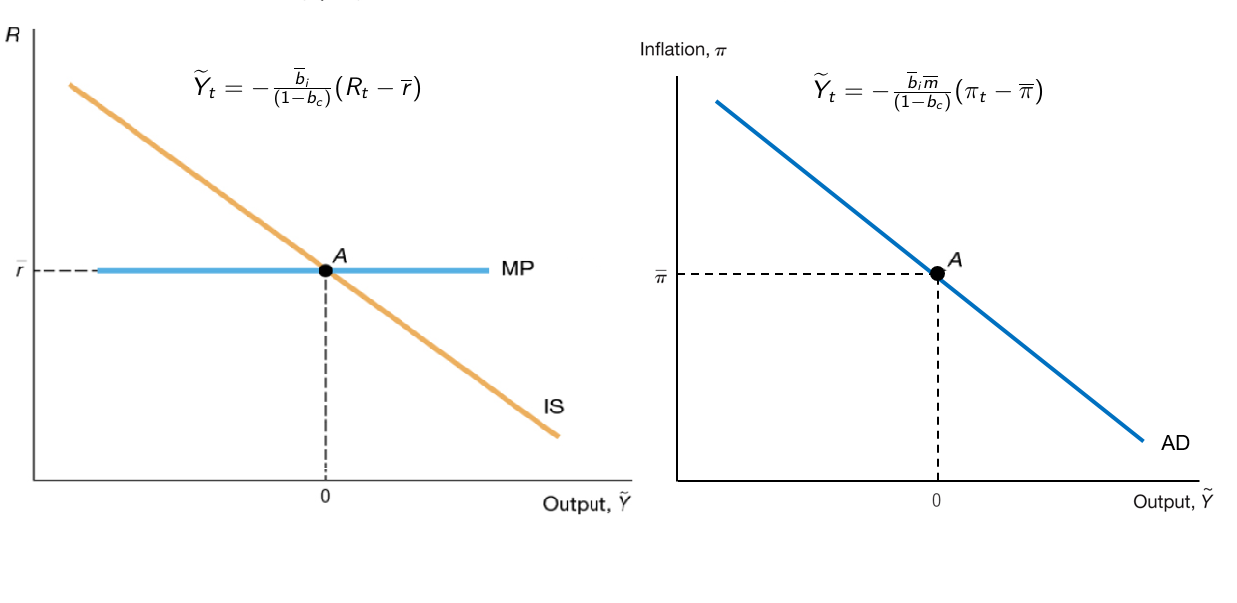
\includegraphics[scale=.35]{ad}
\end{figure}
\end{frame}

\begin{frame}
\frametitle{\: \: \: AD Curve}
\toplinemedium
\begin{figure}
\centering
\caption{Benchmark IS, AD curves (i.e. $\overline{a}=1-b_c$)}
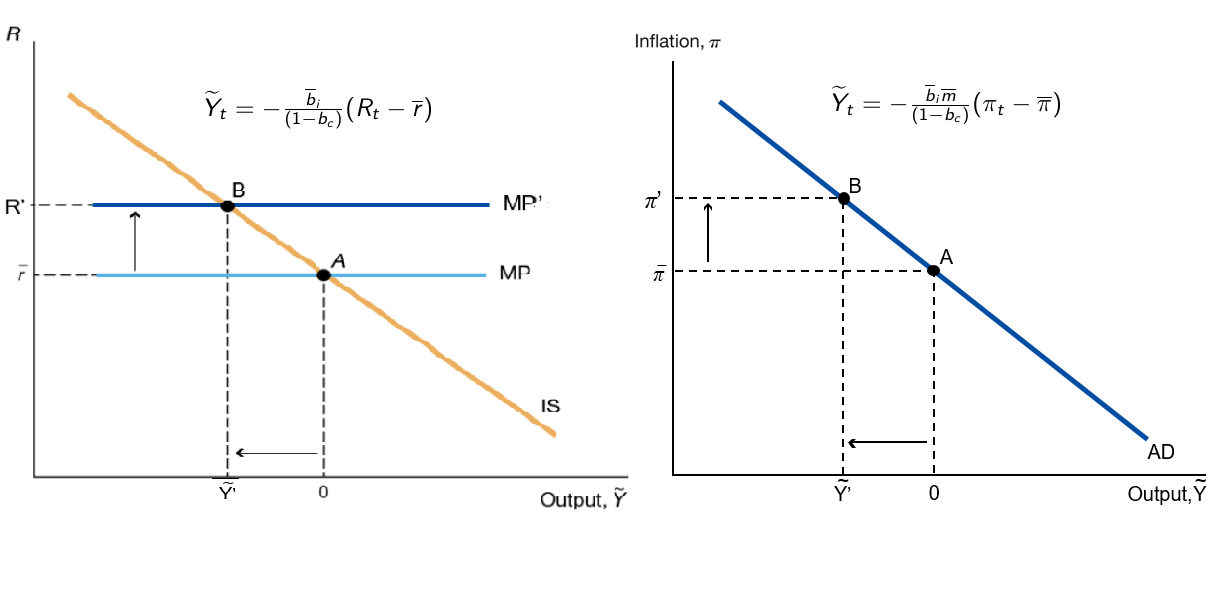
\includegraphics[scale=.35]{ad_2}
\end{figure}
\end{frame}


\begin{frame}
\frametitle{\: \: \: AD Curve}
\toplinemedium
\begin{figure}
\centering
\caption{IS, AD curves ($\overline{a}=1-b_c$, $\overline{a}_1>\overline{a}$)}
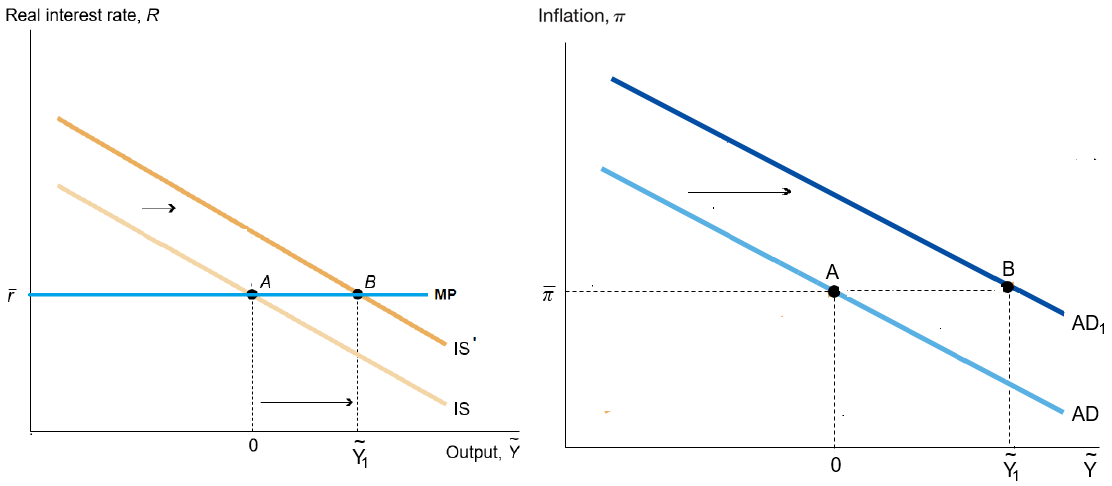
\includegraphics[scale=.38]{ad_3}
\end{figure}
\end{frame}

\begin{frame}
\frametitle{\: \: \: AS Curve}
\toplinemedium
\begin{itemize}
\item We rewrite price setting behaviour from Phillips Curve as:
\begin{eqnarray*}
\begin{array}{ll}
\text{AS Curve:} &\pi_t=\pi_{t-1}+\overline{v}\widetilde{Y}_t+\overline{o}_t
\end{array}
\end{eqnarray*}
\end{itemize}
\end{frame}

\begin{frame}
\frametitle{\: \: \: AS Curve}
\toplinemedium
\begin{figure}
\centering
\caption{Benchmark AS curve (i.e. $\pi_{t-1}=\overline{\pi}$, $\overline{o}_t=0$)}
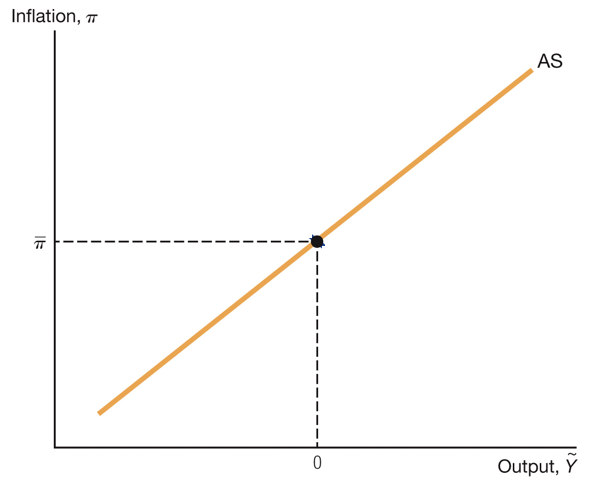
\includegraphics[scale=.45]{as_1}
\end{figure}
\end{frame}

\begin{frame}
\frametitle{\: \: \: AS Curve}
\toplinemedium
\begin{figure}
\centering
\caption{Benchmark AS curve (i.e. $\pi_{t-1}>\overline{\pi}$, $\overline{o}_t=0$)}
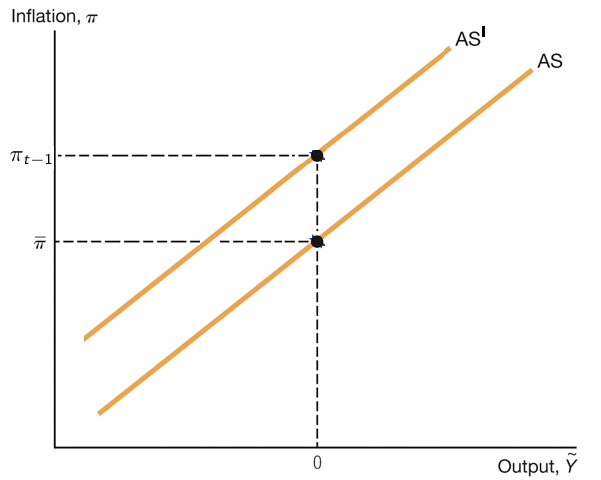
\includegraphics[scale=.45]{as_2}
\end{figure}
\end{frame}


\begin{frame}
\frametitle{\: \: \: AS-AD Model}
\toplinemedium
\begin{figure}
\centering
\caption{Benchmark AS curve ($\pi_{t-1}=\overline{\pi}$, $\overline{o}_t=0$), AD ($\overline{a}=1-b_c$) }
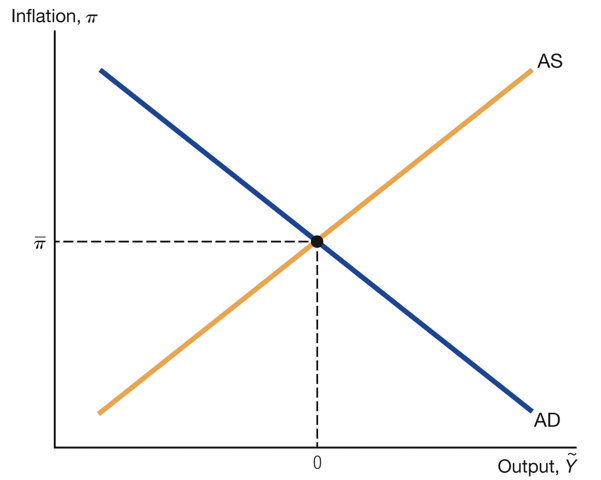
\includegraphics[scale=.45]{as_ad}
\end{figure}
\end{frame}

\section{Using the AS-AD Model}

\begin{frame}
\frametitle{\: \: \: Cost-push Shock}
\toplinemedium
\begin{figure}
\centering
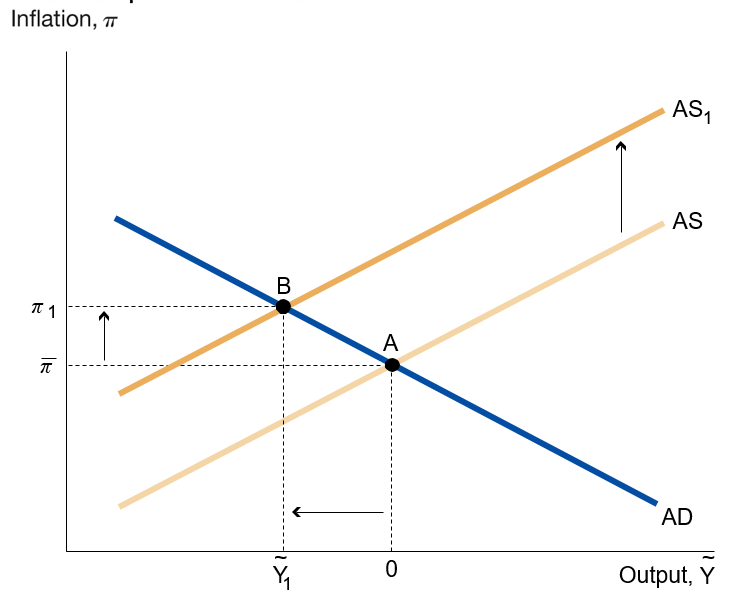
\includegraphics[scale=.45]{AS_AD_inflation}
\end{figure}
\end{frame}

\begin{frame}
\frametitle{\: \: \: Inflation Shock}
\toplinemedium
\begin{figure}
\centering
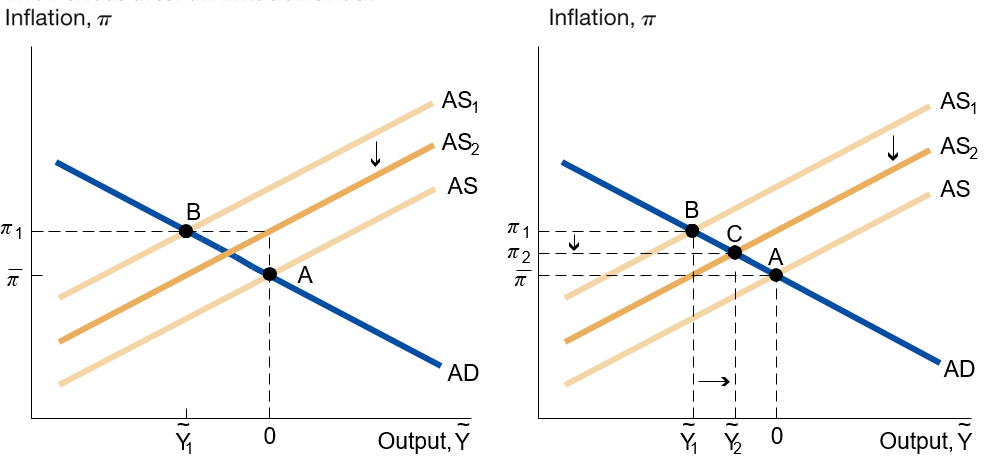
\includegraphics[scale=.45]{AS_AD_inflation_2}
\end{figure}
\end{frame}

\begin{frame}
\frametitle{\: \: \: Cost-push Shock}
\toplinemedium
\begin{figure}
\centering
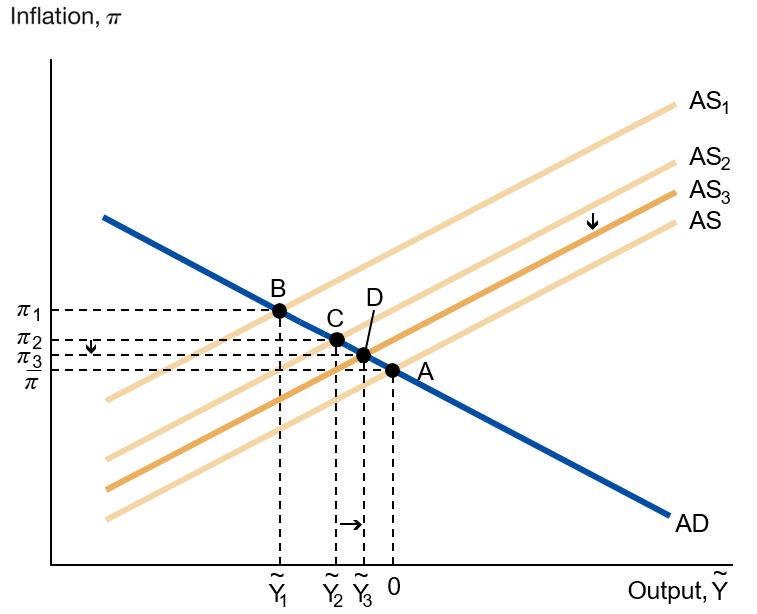
\includegraphics[scale=.45]{AS_AD_inflation_3}
\end{figure}
\end{frame}

\begin{frame}
\frametitle{\: \: \: Cost-push Shock}
\toplinemedium
\begin{figure}
\centering
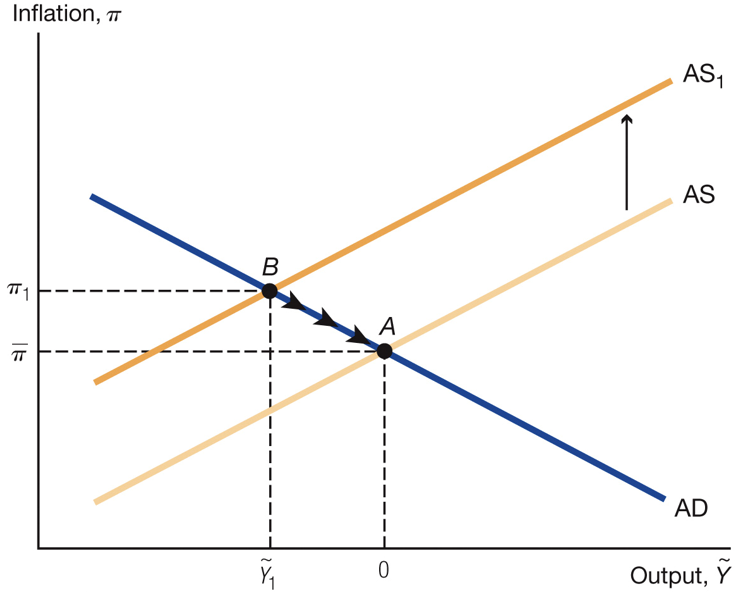
\includegraphics[scale=.45]{AS_AD_inflation_4}
\end{figure}
\end{frame}


\begin{frame}
\frametitle{\: \: \: One Period Demand Shock}
\toplinemedium
\begin{figure}
\centering
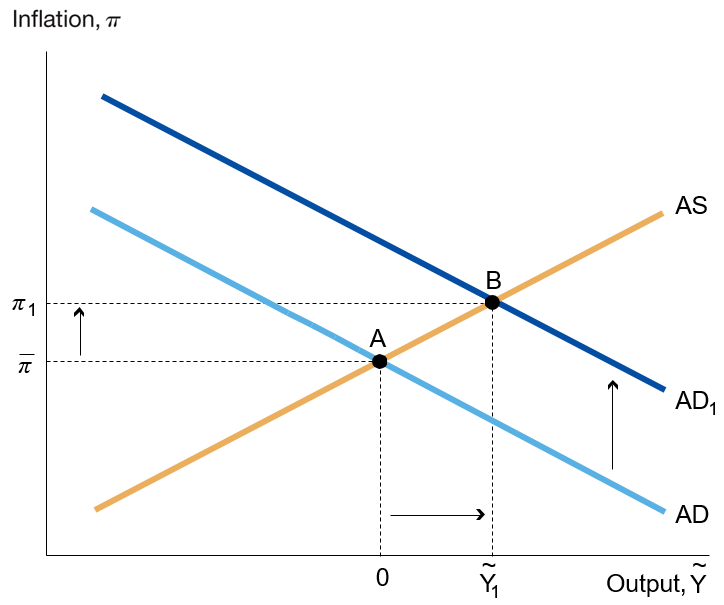
\includegraphics[scale=.45]{demand_shock_1}
\end{figure}
\end{frame}

\begin{frame}
\frametitle{\: \: \: One Period Demand Shock}
\toplinemedium
\begin{figure}
\centering
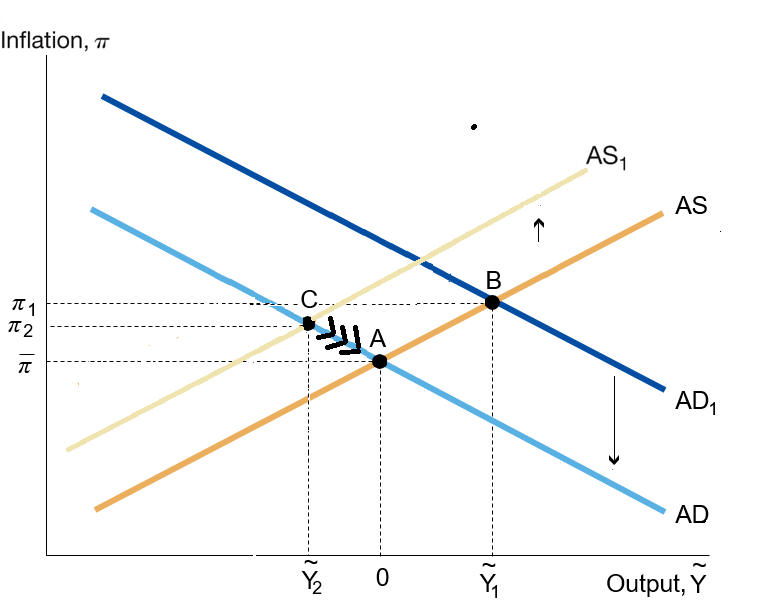
\includegraphics[scale=.45]{demand_shock_2}
\end{figure}
\end{frame}

\begin{frame}
\frametitle{\: \: \: Multiple Period Demand Shock}
\toplinemedium
\begin{figure}
\centering
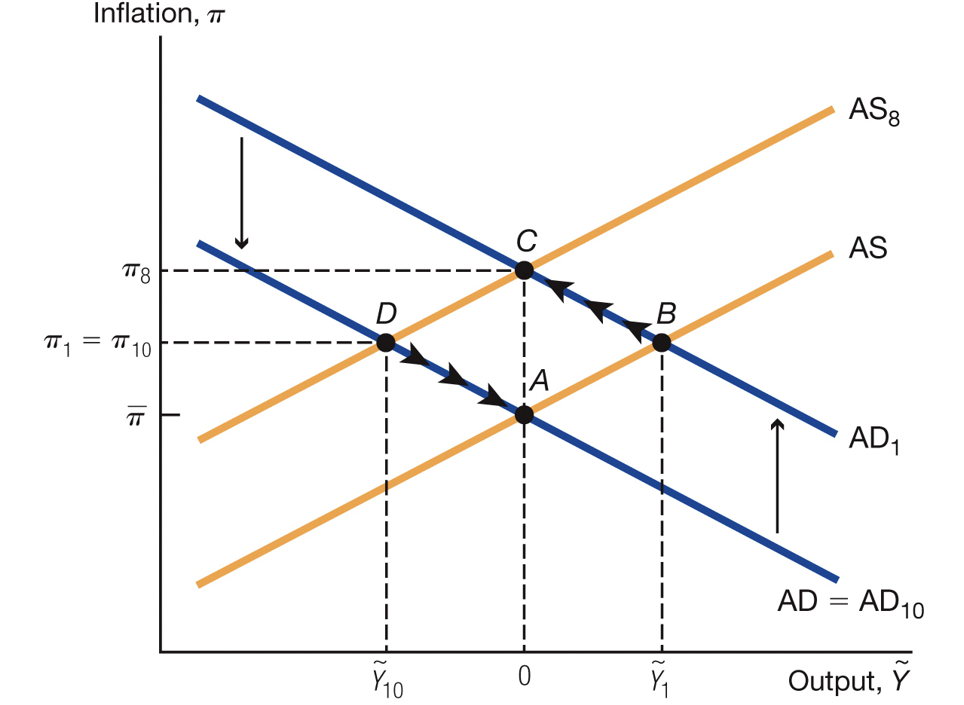
\includegraphics[scale=.35]{demand_shock_3}
\end{figure}
\end{frame}


\begin{frame}
\frametitle{\: \: \: Phase diagram cost push and demand shocks}
\toplinexlarge
\begin{figure}
\centering
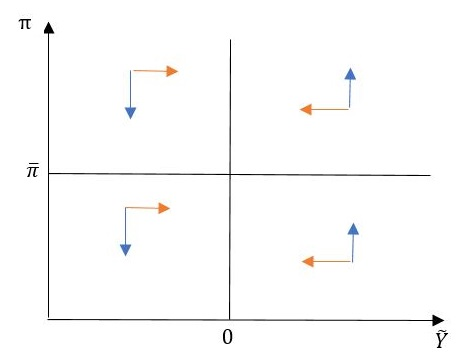
\includegraphics[scale=.67]{phase_diagram}
\end{figure}
\end{frame}



\begin{frame}
\frametitle{\: \: \: Empirical Evidence}
\toplinemedium
\begin{figure}
\centering
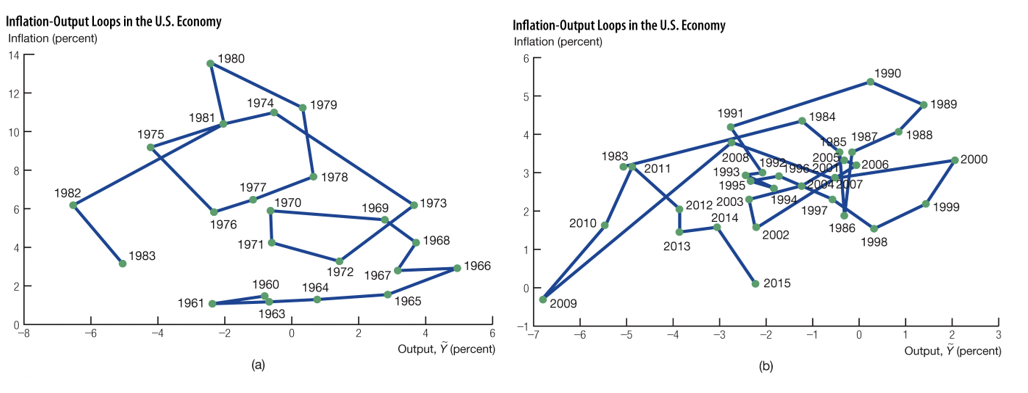
\includegraphics[scale=.4]{empirics}
\end{figure}
\end{frame}

\begin{frame}
\frametitle{\: \: \: Rules vs. Discretion}
\toplinemedium
\begin{itemize}
\item Explicit Policy Rules:
\vspace{0.1in}
\begin{itemize}
\item (pros) Help anchor inflation expectations and maintain a stable inflation environment where shocks are deflected quickly
\vspace{0.1in}
\item (cons) To work, policy rules must be credible, and, therefore, provide little flexibility to deviate from targets
\end{itemize}
\vspace{0.1in}
\item Discretionary Monetary Policy:
\begin{itemize}
\vspace{0.1in}
\item (pros) Provides flexibility to pursue expansionary economic policy
\vspace{0.1in}
\item (cons) Shocks can be very disruptive as inflation pressures do not dissipate quickly
\end{itemize}
\vspace{0.1in}
\item It is extremely important that, in Modern Economies, CBs are independent from the government in power
\end{itemize}
\end{frame}


\end{document}


